\documentclass[17pt]{extreport}

\usepackage[
    paper=a3paper,
    landscape,
  margin=0pt
]{geometry}

% --- PACKAGES ---
\usepackage{booktabs}
\usepackage{array}
\usepackage{multirow}
\usepackage{siunitx}
\usepackage{graphicx}
\usepackage{makecell}
\usepackage{longtable}

% --- GLOBAL CENTERING FOR ALL CELLS ---
\renewcommand{\cellalign}{cc}

\sisetup{
  exponent-product = \cdot,
  output-exponent-marker = e
}

\begin{document}

\begin{center}
\Large\textbf{Summary of Convolutional Autoencoder Runs (3D Case, CDI Method, Diffuse Interface)}
\end{center}

\vspace{1cm}

\small  % reduce text size slightly for better fit

\begin{longtable}{
  >{\centering\arraybackslash}p{91.69574pt}
  >{\centering\arraybackslash}p{157.06654pt}
  >{\centering\arraybackslash}p{104.96567pt}
  >{\centering\arraybackslash}p{148.29828pt}
  >{\centering\arraybackslash}p{90.21239pt}
  >{\centering\arraybackslash}p{95.22563pt}
  >{\centering\arraybackslash}p{56.52945pt}
  >{\centering\arraybackslash}p{102.5522pt}
  >{\centering\arraybackslash}p{154.26381pt}
}
\toprule
Case &
\makecell[c]{Input size and channels \\ $N_c \times N_x \times N_y \times N_z$} &
\makecell[c]{Sample size \\ $N_{TR}$ \\ $N_{VL}$} &
\makecell[c]{Architecture \\ Base dim \\ \texttt{dim\_mult} \\ Channel output} &
\makecell[c]{Latent space \\ CR} &
Learning rate &
Epochs &
ETR &
Notes / Result \\
\midrule
\endfirsthead

% HEADER REPEATED ON NEXT PAGE
\toprule
Case &
\makecell[c]{channels and Input size \\ $N_c \times N_x \times N_y \times N_z$} &
\makecell[c]{Sample size \\ $N_{TR}$ \\ $N_{VL}$} &
\makecell[c]{Architecture} &
\makecell[c]{Latent space \\ CR} &
Learning rate &
Epochs &
Notes &
Result \\
\midrule
\endhead

% ------------------------- CASE 1 -------------------------
1 &
\makecell[c]{$2 \times 64 \times 64 \times 64$ \\ \textcolor{red}{G, V}} &
\makecell[c]{390 \\ $312|78$} &
\makecell[c]{16 \\ (1) \\ (16, 20)} &
\makecell[c]{$20\times64\times64\times64$ \\ $N_z = 20$ \\ CR=0.1} &
$1\times10^{-3}$ &
100 &
$\sim 4$ h &
\makecell[c]{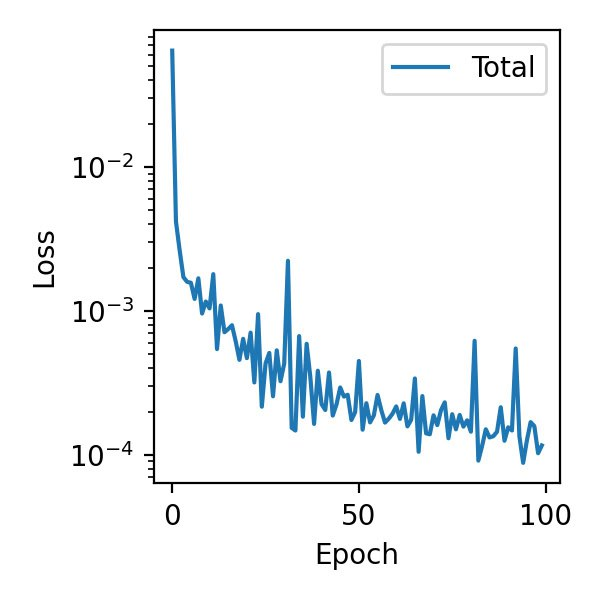
\includegraphics[width=5cm]{1.jpg}} \\
\midrule

% ------------------------- CASE 2 -------------------------
2 &
\makecell[c]{$2 \times 64 \times 64 \times 64$ \\ \textcolor{red}{G, V}} &
\makecell[c]{390 \\ $312|78$} &
\makecell[c]{16 \\ (1,2,4,8) \\ (16,32,64,20)} &
\makecell[c]{$20\times16\times16\times16$ \\ $N_z = 20$ \\ CR=6.4} &
$1\times10^{-3}$ &
100 &
$\sim 9$ h &
\makecell[c]{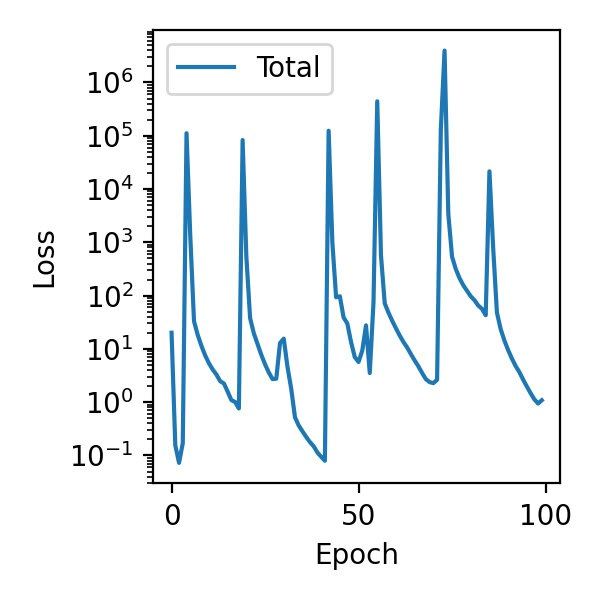
\includegraphics[width=5cm]{2.jpg}} \\
\midrule

% ------------------------- CASE 3 -------------------------
3 &
\makecell[c]{$1 \times 64 \times 64 \times 64$ \\ \textcolor{red}{G}} &
\makecell[c]{390 \\ $312|78$} &
\makecell[c]{16 \\ (1,2,4,8) \\ (16,32,64,20)} &
\makecell[c]{$20\times16\times16\times16$ \\ $N_z = 20$ \\ CR=3.2} &
$1\times10^{-3}$ &
100 &
$\sim 2$ h &
\makecell[c]{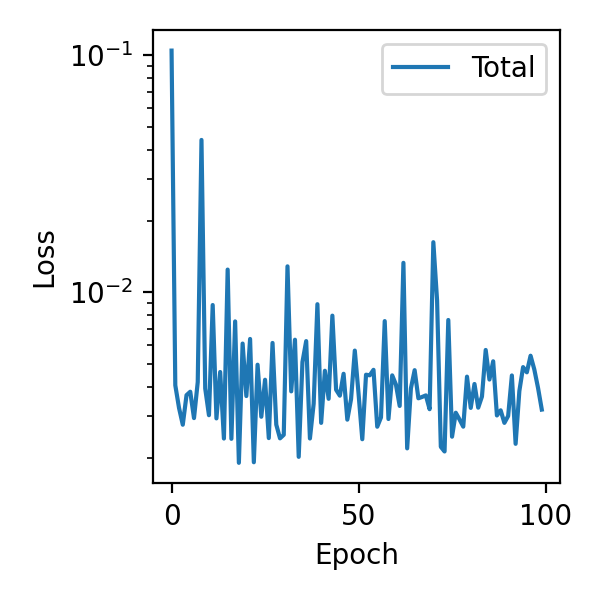
\includegraphics[width=5cm]{3.jpg}} \\
\midrule

% ------------------------- CASE 4 -------------------------
4 &
\makecell[c]{$1 \times 64 \times 64 \times 64$ \\ \textcolor{red}{G}} &
\makecell[c]{390 \\ $312|78$} &
\makecell[c]{16 \\ (1,2,4,8,16,32,64,128) \\ (16,32,64,128,256,512,1024,10)} &
\makecell[c]{$10\times1\times1\times1$ \\ $N_z = 10$ \\ CR=26214.4} &
$1\times10^{-4}$ &
100 &
\makecell[c]{$\sim 2$ h \\ 2×V100 32GB GPUs} &
\makecell[c]{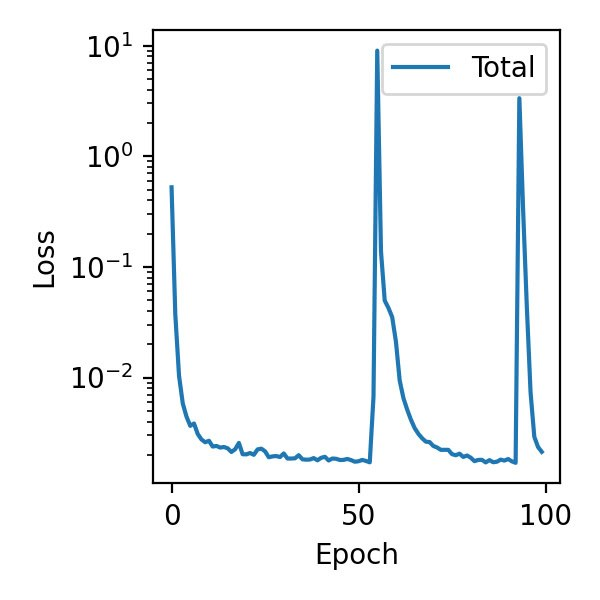
\includegraphics[width=5cm]{4.jpg}} \\
\midrule

% ------------------------- CASE 5 -------------------------
\makecell[c]{5 \\ 3DMPF \\ datasets} &
\makecell[c]{$1 \times 128 \times 256 \times 128$ \\ \textcolor{red}{G}} &
\makecell[c]{918 \\ $734|184$} &
\makecell[c]{16 \\ (1,2,4,8,16,32,64) \\ (16,32,64,128,512,16)} &
\makecell[c]{$16\times4\times8\times4$ \\ $N_z = 16$ \\ CR=2048} &
$1\times10^{-4}$ &
100 &
\makecell[c]{12hrs \\ A100 80GB \\ Batch size = 2} &
\makecell[c]{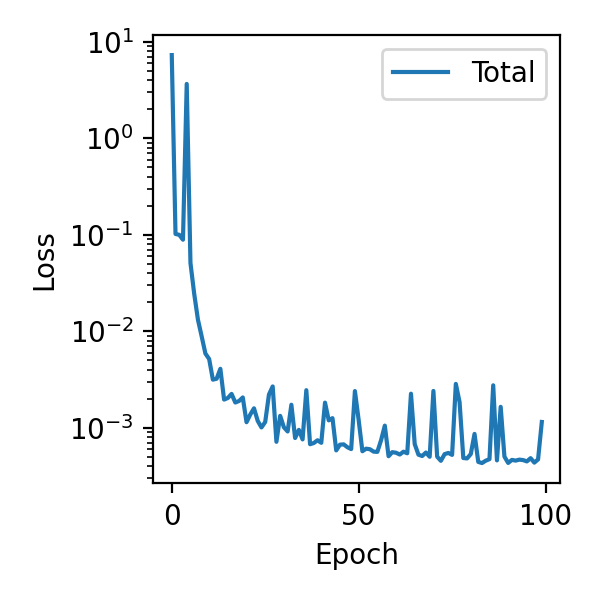
\includegraphics[width=5cm]{5.png}} \\
\midrule

% ------------------------- CASE 6 -------------------------
\makecell[c]{6 \\ 3DMPF \\ datasets} &
\makecell[c]{$1 \times 128 \times 256 \times 128$ \\ \textcolor{red}{G}} &
\makecell[c]{918 \\ $734|184$} &
\makecell[c]{16 \\ (1,2,4,8,16,32,64) \\ (16,32,64,128,512,16)} &
\makecell[c]{$16\times4\times8\times4$ \\ $N_z = 16$ \\ CR=2048} &
$1\times10^{-4}$ &
100 &
\makecell[c]{\textcolor{red}{23hrs} \\ A100 80GB \\ \textcolor{red}{Batch size = 4}} &
\makecell[c]{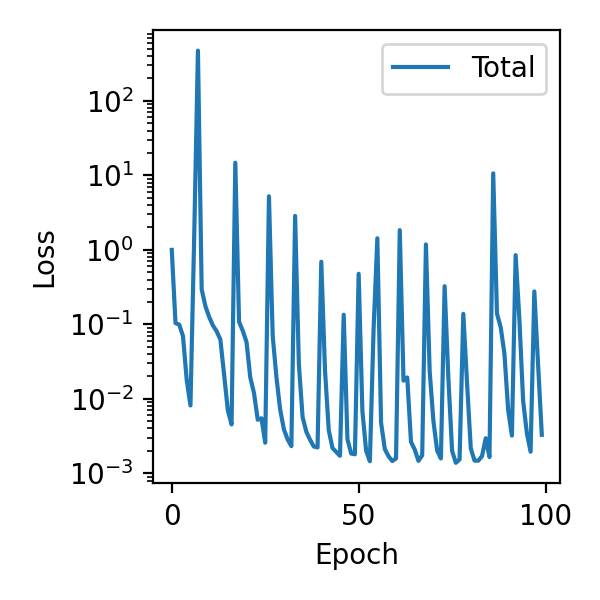
\includegraphics[width=5cm]{6.png}} \\
\midrule

% ------------------------- CASE 7 -------------------------
\makecell[c]{7 \\ 3DMPF \\ datasets} &
\makecell[c]{$1 \times 128 \times 256 \times 128$ \\ \textcolor{red}{G}} &
\makecell[c]{918 \\ $734|184$} &
\makecell[c]{16 \\ (1,2,4,8,16,32,64) \\ (16,32,64,128,512,16)} &
\makecell[c]{$16\times4\times8\times4$ \\ $N_z = 16$ \\ CR=2048} &
\textcolor{red}{$1\times10^{-5}$} &
100 &
\makecell[c]{\textcolor{red}{23hrs} \\ A100 80GB \\ \textcolor{red}{Batch size = 4}} &
\makecell[c]{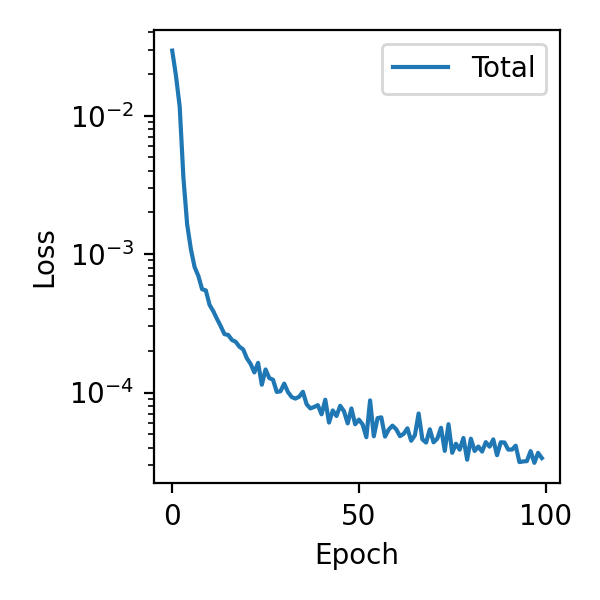
\includegraphics[width=5cm]{7.png}} \\
\midrule


% ------------------------- CASE 8 -------------------------
\makecell[c]{8 \\ 2DMPF \\ datasets} &
\makecell[c]{$1 \times 1 \times 512 \times 256$ \\ \textcolor{red}{G}} &
\makecell[c]{2400 \\ $1920|480$} &
\makecell[c]{16 \\ (1,2,4,8,16,32,64,128) \\ (16,32,64,128,256,512,1024,4)} &
\makecell[c]{$4\times8\times4$ \\ $N_z = 4$ \\ CR=1024} &
$1\times10^{-5}$ &
100 &
\makecell[c]{\textcolor{black}{5hrs} \\ A100 40GB \\ \textcolor{black}{Batch size = 16}} &
\makecell[c]{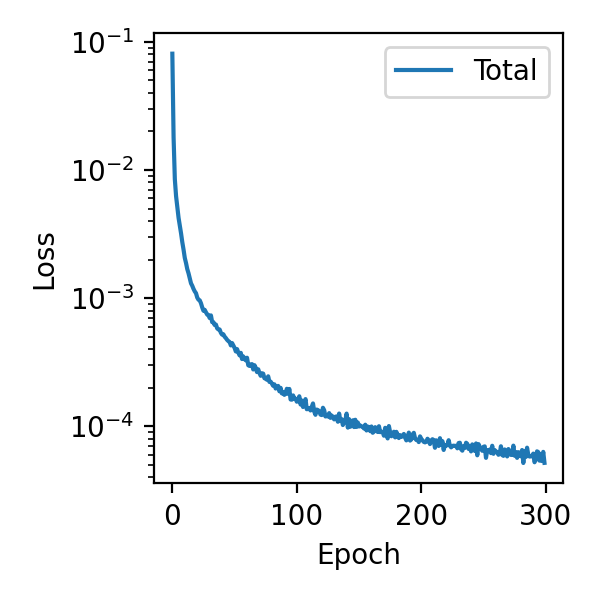
\includegraphics[width=5cm]{8.png}} \\
\midrule

% ------------------------- CASE 9 -------------------------
\makecell[c]{9 \\ 2DMPF \\ datasets} &
\makecell[c]{$3 \times 512 \times 256 \times 1$ \\ \textcolor{red}{G, V, W}} &
\makecell[c]{2400 \\ $1920$\\$480$} &
\makecell[c]{Resent-CAE \\ Base dim=16 \\8 Layers\\(1,2,4,8,16,32,64,128)\\(16,32,64,128,256,512,1024,4)} &
\makecell[c]{$4\times8\times4$ \\ \textcolor{red}{CR=3072}} &
$1\times10^{-5}$ &
100 &
\makecell[c]{\textcolor{black}{5hrs} \\ A100 \textcolor{red}{80Gb} \\ \textcolor{black}{Batch size = 16}} &
\makecell[c]{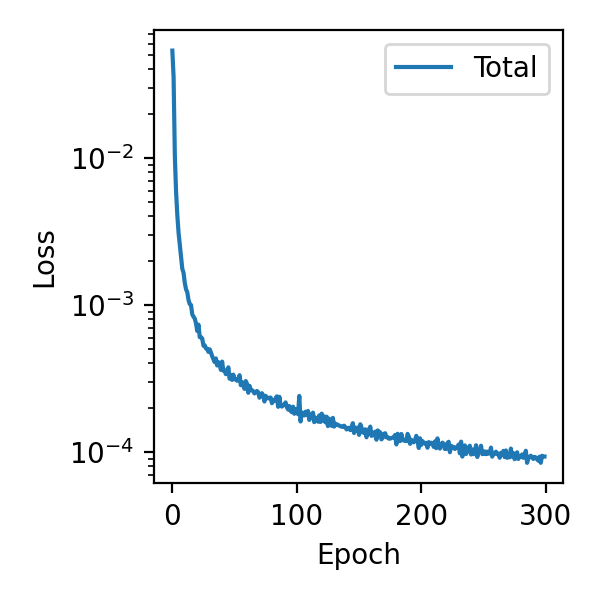
\includegraphics[width=5cm]{9.png}} \\
\midrule


% ------------------------- CASE 10 -------------------------
\makecell[c]{10 \\ 2DAdvection \\ datasets} &
\makecell[c]{$1 \times 256 \times 256 \times 1$ \\ \textcolor{red}{u}} &
\makecell[c]{$79\times16=1264$ \\ $15\times16=240$ \\ $64\times16=1024$} &
\makecell[c]{Resent-CAE\\ Base dim=16 \\ 6 Layers \\ (1,2,4,8,16,32) \\ (16,32,64,128,256,4)} &
\makecell[c]{$4\times16\times16$ \\ \textcolor{red}{CR=64}} &
$1\times10^{-5}$ &
300 &
\makecell[c]{\textcolor{black}{1.5hrs} \\ T100 \textcolor{red}{8Gb} \\ \textcolor{black}{Batch size = 8}} &
\makecell[c]{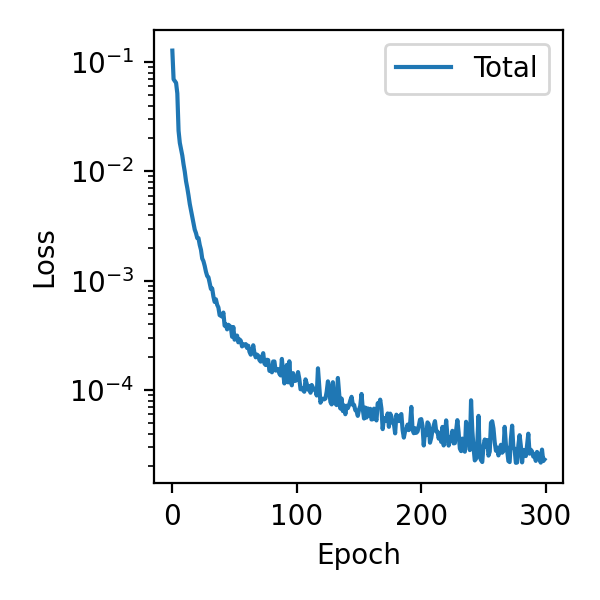
\includegraphics[width=5cm]{10.png}} \\
\midrule


% ------------------------- CASE 11 -------------------------
\makecell[c]{11 \\ 2DAdvection \\ datasets} &
\makecell[c]{$1 \times 256 \times 256 \times 1$ \\ \textcolor{red}{u}} &
\makecell[c]{$79\times16=1264$ \\ $15\times16=240$ \\ $64\times16=1024$} &
\makecell[c]{Wang (simple)-CAE\\ Base dim=16 \\ 6 Layers \\ (1,2,4,8,16,32) \\ (16,32,64,128,256,512)} &
\makecell[c]{$4$ \\ \textcolor{red}{CR=16384}} &
$1\times10^{-4}$ &
5000 &
\makecell[c]{\textcolor{black}{3hrs} \\ T100 \textcolor{red}{8Gb} \\ \textcolor{black}{Batch size = 8} \\ early stop, 500} &
\makecell[c]{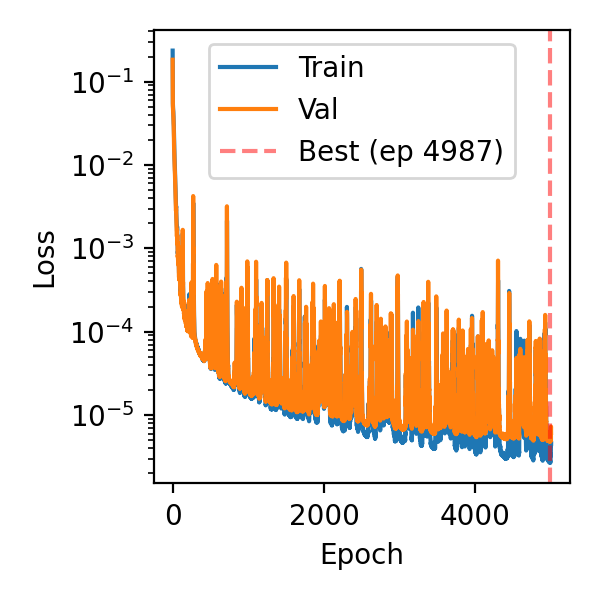
\includegraphics[width=5cm]{11.png}} \\
\midrule

\bottomrule

\end{longtable}



\vspace{2cm}

\section{MPF Sample Dataset: 10 Simulations (Phase-Field Model)}

\noindent In total, there are \textbf{500 simulations}, each containing \textbf{51 snapshots}. \\

\noindent\textbf{Case properties:}
\[
X = [\rho^*,\, \mu^*,\, Bo,\, Re], \qquad 
Y = [c,\, u,\, v,\, w,\, P,\, \rho]
\]

\noindent\textbf{Property ranges:}
\[
\rho^* \in [10,\,1000], \qquad
\mu^* \in [1,\,100], \qquad
Bo \in [10,\,500], \qquad
Re \in [10,\,500]
\]

\noindent\textbf{3D dataset shape:}
\[
[\,n_t = 10,\; \text{channels} = 6,\; n_x = 256,\; n_y = 256,\; n_z = 256\,]
\]

\noindent The actual spatial resolution
\[
[128,\; 256,\; 128]
\]

\vspace{0.5cm}

\noindent\textbf{Key questions:}
\begin{enumerate}
    \item Should we consider the entire domain, or only the box surrounding the bubble? \textcolor{red}{The entire domain}
    \item If we use the full domain, should the snapshots be fed to the autoencoder in batches or as a single input block? \textcolor{red}{as a single block}
    \item Which bubbles should be included during training? Should cases involving bubble breakup also be considered? \textcolor{red}{DR and VR are fixed (=10, as in 3D cases we have) and vary the Re and BO numbers}
    \item After training a well-performing autoencoder, should we test it on our own dataset?
\end{enumerate}


\begin{longtable}{c c c c c c c c c}
	\toprule
	Case &
	\makecell[c]{Physical parameters} &
	\makecell[c]{Sample size \\ $N_{TR}$ \\ $N_{VL}$} &
	\makecell[c]{Architecture} &
	\makecell[c]{Latent space from CAE} &
	Learning rate &
	Epochs &
	ETR &
	Notes / Result \\
	\midrule
	\endfirsthead
	
	% HEADER REPEATED ON NEXT PAGE
	\toprule
	Case &
	\makecell[c]{channels and Input size \\ $N_c \times N_x \times N_y \times N_z$} &
	\makecell[c]{Sample size \\ $N_{TR}$ \\ $N_{VL}$} &
	\makecell[c]{Architecture} &
	\makecell[c]{Latent space \\ CR} &
	Learning rate &
	Epochs &
	Notes &
	Result \\
	\midrule
	\endhead
	
	  % ------------------------- CASE 9* -------------------------
	\makecell[c]{9* \\ 2DMPF \\ datasets} &
	\makecell[c]{$5$ \\ \textcolor{red}{$(DR, VR, Re, Eo, t)$}} &
	\makecell[c]{$2400$ \\ $1920$ \\ $480$} &
	\makecell[c]{H=64 \\ 3 Layers} &
	\makecell[c]{$4\times8\times4$ \\ \textcolor{red}{CR=64}} &
	$1\times10^{-3}$ &
	5000 &
	\makecell[c]{\textcolor{black}{20 secs} \\ T100 \textcolor{red}{8Gb} \\ \textcolor{black}{Batch size = 32} \\ early stop, 500} &
	\makecell[c]{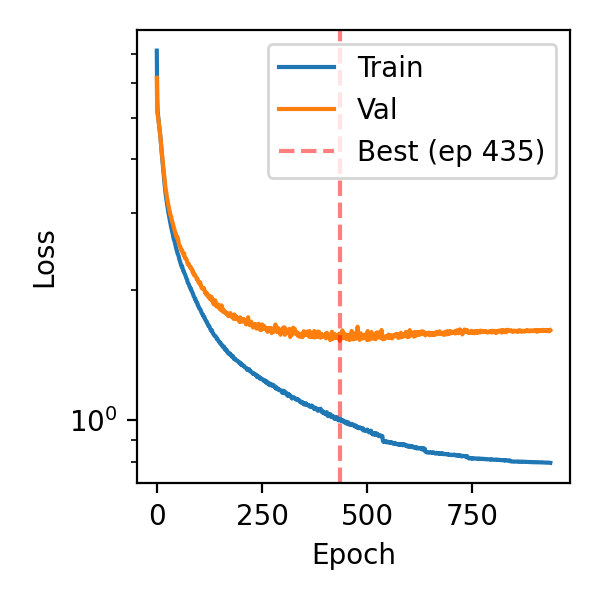
\includegraphics[width=5cm]{9s.png}} \\
	\midrule
	
	% ------------------------- CASE 10* -------------------------
	\makecell[c]{10* \\ 2DAdvection \\ datasets} &
	\makecell[c]{$2$ \\ \textcolor{red}{$(\mu, t)$}} &
	\makecell[c]{$79\times16=1264$ \\ $15\times16=240$ \\ $64\times16=1024$} &
	\makecell[c]{H=64 \\ 3 Layers} &
	\makecell[c]{$4\times16\times16$ \\ \textcolor{red}{CR=64}} &
	$1\times10^{-3}$ &
	5000 &
	\makecell[c]{\textcolor{black}{20 secs} \\ T100 \textcolor{red}{8Gb} \\ \textcolor{black}{Batch size = 32} \\ early stop, 500} &
	\makecell[c]{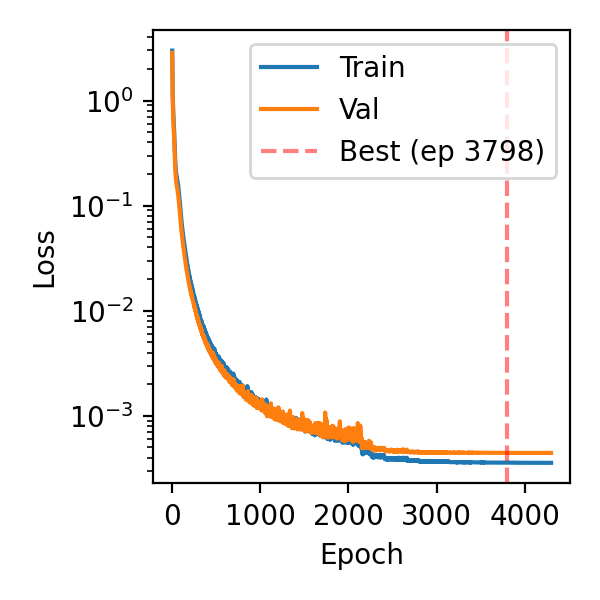
\includegraphics[width=5cm]{10s.png}} \\
	\midrule
	
	\bottomrule
	
	

	
	\bottomrule
\end{longtable}


\begin{center}
	\Large\textbf{Summary of CNN (MLP) Runs}
\end{center}








\end{document}
